\documentclass[11pt]{article}

\usepackage{graphicx}
\usepackage{amsmath}
\usepackage{textcomp}
\usepackage[top=0.8in, bottom=0.8in, left=0.8in, right=0.8in]{geometry}
% Add other packages here %



% Put your group number and names in the author field %
\title{\bf Exercise 1.\\ Implementing a first Application in RePast: A Rabbits Grass Simulation.}
\author{Group \textnumero: 14; Launay Clement}

\begin{document}
\maketitle

\section{Implementation}
\subsection{Assumptions}
% Describe the assumptions of your world model and implementation (e.g. is the grass amount bounded in each cell) %

In addition to the requirements given in the exercise statement, the following assumptions and choices have been made:

\begin{itemize}

\item Rabbits' energy : Rabbits start with a set given number of energy which can be modified with the variable \textit{initialEnergy}.
 
\item Grass : As suggested by NetLogo simulation, each patch of grass is worth a certain amount of energy. It is controlled by the variable \textit{grassValue}. With the requested \textit{grassGrowthRate}, it allows for more precise tuning. It is also assumed that grass can spawn anywhere on the grid at any time, increasing the worth of a cell in energy if it happens to already contains some grass. There is no limit to the amount of grass one cell can contains. However, rabbits always eat all the grass available on the cells they move to.
 
\item Rabbits' collisions: Considering that newborn rabbits should randomly be added to the grid but cannot overlap with others, the method responsible for this, \textit{addNewRabbit} may fail if it does not find an appropriate space after a certain number of tries. In that case there are likely very few spots actually available, so the number of rabbits is too high to be affected. Another issue is rabbits trying to move to a cell already occupied by another rabbit. In that case they do not get to pick another destination and simply do not move for this turn (they still lose energy though).

\end{itemize}

\subsection{Implementation Remarks}
% Provide important details about your implementation, such as handling of boundary conditions %

\begin{itemize}


\item Schedule order: The different part of the \textit{step} function are resolved in the following order.
\begin{enumerate}
\item A \textit{grassGrowthRate} number of patches of grass are randomly added to the space.
\item One after the other, each rabbit eats all the grass at its position, gaining the corresponding energy, then choose a random direction to move in, effectively moving if the destination cell is free, and loose one energy
\item Each rabbit is checked to see if it has died (energy=0) and should be remove, or if it should give birth, reducing its energy and adding a new rabbit in the space.     
\end{enumerate}


\item Movements : Rabbits move by picking a random number between 0 and 3 which tell them how they should try to modify their coordinates (e.g. $0\longrightarrow NORTH \longrightarrow (0,1) \longrightarrow (x+0,y+1)$). They can then compute their destination's coordinates with a modulus to comply with the torus space design and request the simulation space to handle the movement.

\item Simulation feedback : Alongside the simulation, two plots display the evolution of the rabbit population and the amount of grass energy available on the field. They have separated windows because their scales can greatly vary depending on the simulation's parameters. It is also possible to access and modify the details of any given cell by clicking on them. On the display, rabbits are represented by white circles while cells with grass are colored with brown when empty and with darker and darker shades of green as their amount of grass increase (up to black when they reach 16 patches).

\end{itemize}

\section{Results}
% In this section, you study and describe how different variables (e.g. birth threshold, grass growth rate etc.) or combinations of variables influence the results. Different experiments with diffrent settings are described below with your observations and analysis

\subsection{Experiment 1}

\subsubsection{Setting}

\centerline{
\begin{tabular}{|c|c||c|c|}
\hline 
birthCost & 50 & gridSize & 20 \\ 
\hline 
birthThreshold & 100 & initialEnergy & 50\\ 
\hline 
grassGrowthRate & 15 & numberRabbitsInit & 20 \\ 
\hline 
grassValue & 5 & &\\ 
\hline 
\end{tabular}
}

A simple experiment with the default values to observe the evolution of the model. The parameters related to birth are a bit intuitive with $initialEnegery+birthCost=birthThreshold$

\subsubsection{Observations}
% Elaborate on the observed results %

The evolution of the grass and rabbit populations first undergo a transient phase. At the beginning grass have a small window where its number reaches its peak because it is not spread everywhere while rabbits are underpopulated. Since rabbits move at random, they actually rely on grass spawning near them than moving to it. This quickly happens and the number of rabbits then skyrockets (all rabbits tend to give birth at around the same time). Both populations then stabilize, with the final number of rabbits being around 74. The final regime is still subject to small oscillations, clearly visible on the rabbit graph (grass graph is more edgy because rabbits eat all grass in a cell). They are due to the model being unstable by nature: it is a predator-prey systems where the rabbit population grows until it surpass grass's natural growth, at which point some rabbits dies from the lack of grass, allowing more grass to grow since there are now less rabbits, and the cycle starts again. This is coherent with the final average rabbit population being close to $75=15*5=GRASSGROWTHRATE*GRASSVALUE$  

\centerline{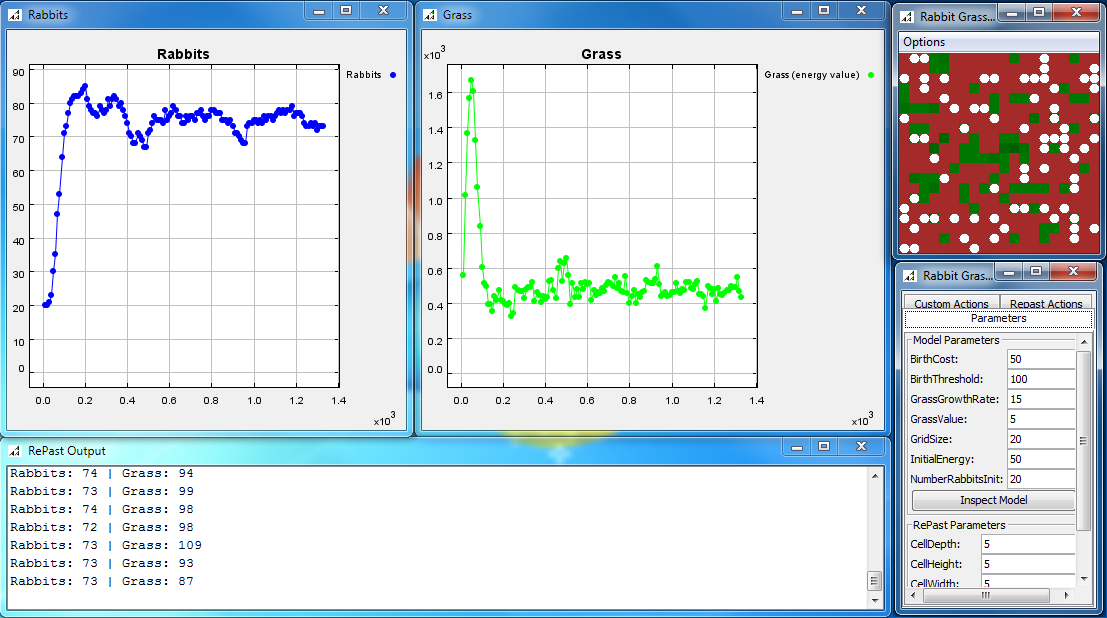
\includegraphics[height=60mm]{exp1.PNG}}



\subsection{Experiment 2}

\subsubsection{Setting}

\centerline{
\begin{tabular}{|c|c||c|c|}
\hline 
birthCost & 50 & gridSize & 20 \\ 
\hline 
birthThreshold & 100 & initialEnergy & 50\\ 
\hline 
grassGrowthRate & 15 & numberRabbitsInit & 30 \\ 
\hline 
grassValue & 1 & &\\ 
\hline 
\end{tabular}
}

\subsubsection{Observations}
% Elaborate on the observed results %
In this experiment, the initial number of rabbits is deliberately higher than the available grass production. Hence the rabbit population starts by declaiming, which is further guaranteed by the \textit{grassValue} being 1 (so rabbits are very unlikely to be able to reproduce before most of them went extinct, allowing path of grass to start being actually worth more than the cost of moving to them). We can then see the establishment of the stable regime with damped oscillations (that will not actually fully disappear).

\centerline{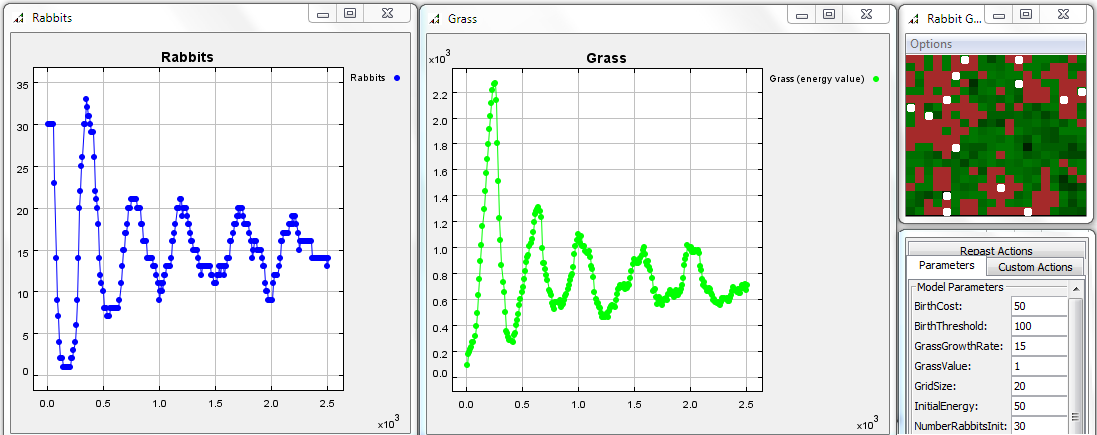
\includegraphics[height=40mm]{exp2.PNG}}


\subsection{Experiment 3}

\subsubsection{Setting}

\centerline{
\begin{tabular}{|c|c||c|c|}
\hline 
birthCost & 5 & gridSize & 40 \\ 
\hline 
birthThreshold & 60 & initialEnergy & 50\\ 
\hline 
grassGrowthRate & 15 & numberRabbitsInit & 20 \\ 
\hline 
grassValue & 5 & &\\ 
\hline 
\end{tabular}
}
These values where found by tinkering with the parameters to obtain the wanted result.

\subsubsection{Observations}
% Elaborate on the observed results %
This experiment features more extreme values for the variable in order to emphasis the inherent instability of this simulation. The results are opposite harmonic oscillations for both populations

\centerline{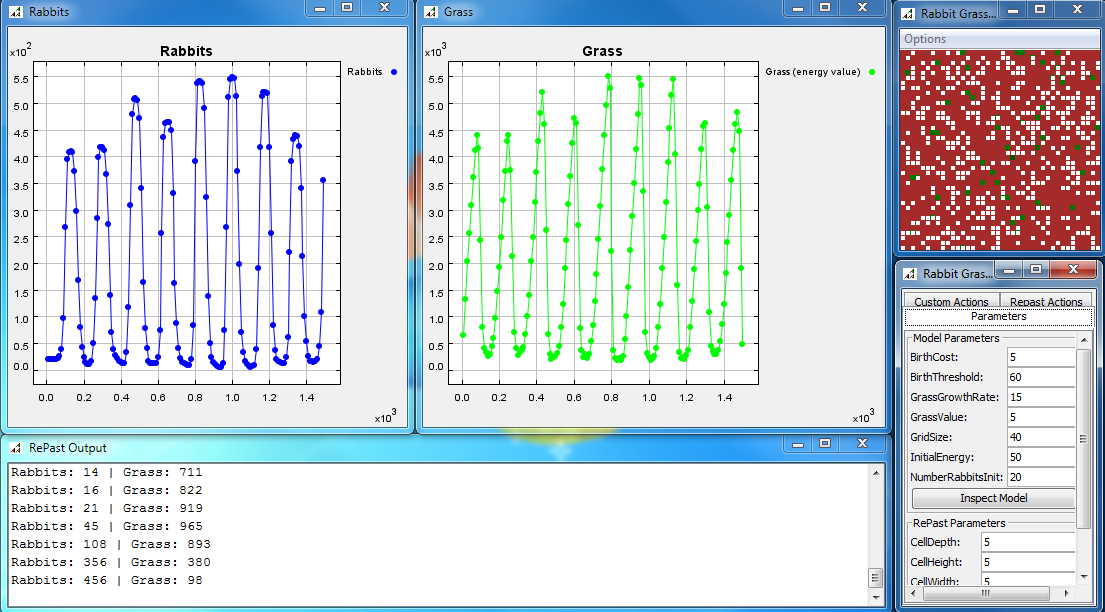
\includegraphics[height=60mm]{exp3.PNG}}

\end{document}